\documentclass[border=6pt]{standalone}
% Shared preamble for web figures.  Each figure is a standalone .tex that
% \input's this file; scripts/make-figures.sh turns it into an SVG.
% Handouts pull the same file with \fig{Unit_X/<name>}.
\usepackage[T1]{fontenc}
\usepackage{helvet}
\renewcommand{\familydefault}{\sfdefault}
\renewcommand{\ttdefault}{pcr}  % Courier: a real Type 1 typewriter font
\usepackage{amsmath}
\usepackage{tikz}
\usetikzlibrary{arrows.meta,positioning,calc,shapes.symbols,shapes.geometric}

% Who makes the rules is the point of most diagrams in this book, so the
% colors mean the same thing everywhere: blue is a person, orange is the
% computer, green is an answer, pink is the human brain.
\definecolor{person}{HTML}{2C6FAE}
\definecolor{machine}{HTML}{D35400}
\definecolor{result}{HTML}{1E8449}
\definecolor{brainpink}{HTML}{C2185B}
\definecolor{ink}{HTML}{2C3E50}

\tikzset{
  doodle/.style={line width=1.5pt, line cap=round, line join=round, draw=ink},
  box/.style={draw, rounded corners=5pt, line width=1.1pt, align=center,
              inner sep=7pt, minimum height=1.0cm, font=\small},
  personbox/.style={box, draw=person, fill=person!10},
  machinebox/.style={box, draw=machine, fill=machine!10},
  resultbox/.style={box, draw=result, fill=result!10},
  plainbox/.style={box, draw=ink!70, fill=ink!4},
  flow/.style={-{Stealth[length=8pt]}, line width=1.4pt, draw=ink},
}

% A person (blue) and a robot head (orange) as small icons.
% \personicon{x}{y}{scale}   \roboticon{x}{y}{scale}
\newcommand{\personicon}[3]{%
  \begin{scope}[shift={(#1,#2)}, scale=#3]
    \fill[person] (0,0.62) circle (0.28);
    \fill[person, rounded corners=6pt] (-0.42,-0.55) rectangle (0.42,0.28);
  \end{scope}}
\newcommand{\roboticon}[3]{%
  \begin{scope}[shift={(#1,#2)}, scale=#3]
    \draw[machine, line width=1.2pt] (0,0.5) -- (0,0.72);
    \fill[machine] (0,0.78) circle (0.08);
    \draw[machine, line width=1.4pt, fill=machine!12, rounded corners=4pt] (-0.5,-0.45) rectangle (0.5,0.5);
    \fill[ink] (-0.2,0.12) circle (0.08);
    \fill[ink] (0.2,0.12) circle (0.08);
    \draw[ink, line width=1pt] (-0.22,-0.22) -- (0.22,-0.22);
  \end{scope}}

\begin{document}
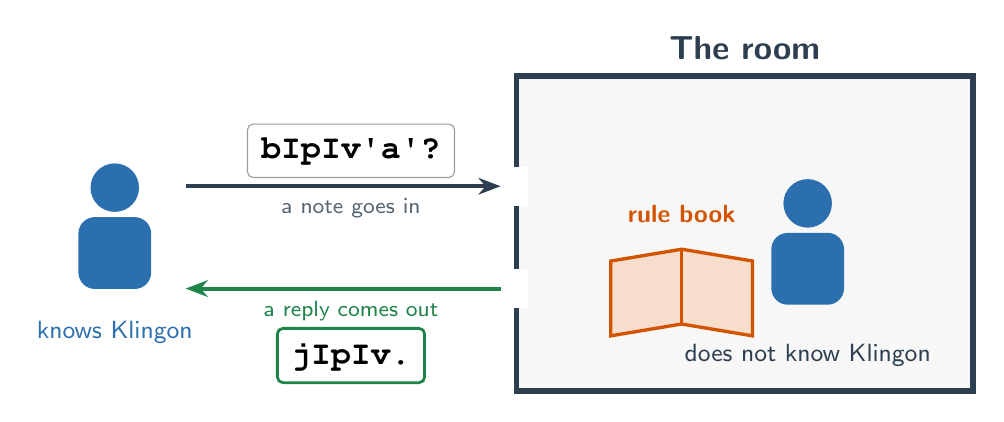
\begin{tikzpicture}
% Searle's Chinese Room (1980), played in Klingon.  A note goes in; the
% person inside follows the rule book and sends back a reply.  They do not
% know Klingon.
\newcommand{\kl}[1]{{\ttfamily\large\bfseries #1}}

% the room
\draw[ink, line width=2pt, fill=ink!4] (3.2,-1.6) rectangle (9.0,2.4);
\node[font=\large\bfseries, text=ink] at (6.1,2.75) {The room};
\fill[white] (3.05,0.75) rectangle (3.35,1.25);  % slot in
\fill[white] (3.05,-0.55) rectangle (3.35,-0.05); % slot out

% person inside with a rule book
\personicon{6.9}{0.1}{1.1}
\draw[machine, line width=1.2pt, fill=machine!20] (4.4,-0.9) -- (5.3,-0.75) -- (6.2,-0.9) -- (6.2,0.05) -- (5.3,0.2) -- (4.4,0.05) -- cycle;
\draw[machine, line width=1.2pt] (5.3,-0.75) -- (5.3,0.2);
\node[font=\small\bfseries, text=machine, align=center] at (5.3,0.65) {rule book};
\node[font=\small, align=center, text=ink] at (6.9,-1.15) {does not know Klingon};

% outside: someone who knows the language
\personicon{-1.9}{0.3}{1.1}
\node[font=\small, align=center, text=person] at (-1.9,-0.85) {knows Klingon};

% note in, reply out
\node[draw=ink!50, fill=white, rounded corners=2pt, inner sep=5pt] at (1.1,1.45) {\kl{bIpIv\textquotesingle{}a\textquotesingle{}?}};
\draw[flow] (-1.0,1.0) -- (3.0,1.0);
\node[font=\footnotesize, text=ink!80] at (1.1,0.72) {a note goes in};
\node[draw=result, fill=white, rounded corners=2pt, inner sep=5pt, line width=1pt] at (1.1,-1.15) {\kl{jIpIv.}};
\draw[flow, draw=result] (3.0,-0.3) -- (-1.0,-0.3);
\node[font=\footnotesize, text=result] at (1.1,-0.58) {a reply comes out};
\end{tikzpicture}
\end{document}
